% !TeX program = lualatex

% setup
\documentclass[
hyperref={bookmarks=false},
xcolor={dvipsnames,svgnames*,x11names*}, 
12pt
]{beamer}
\usepackage{../beamertheme/beamerinnerthemetb}
\usepackage{../beamertheme/beamerouterthemetb}
\usepackage{../beamertheme/beamercolorthemetb}
\usepackage{../beamertheme/beamerthemetb}

% packages
\usepackage{emoji}
\usepackage{graphicx}
\usepackage{xurl}
\usepackage{epigraph}
\setlength\epigraphwidth{\linewidth}

% options
\setlength{\leftmargini}{0.08cm}
\hypersetup{
  pdfauthor={Andrea Gilardi},
  colorlinks=true,
  urlcolor=Blue
}

% metadata
\title{R4DS - Unit 1: Tidyverse}
\author{Andrea Gilardi}
\date{\today}

%%% Define new stuff for slide numbers
\setbeamertemplate{navigation symbols}{}

\pgfkeys{/visual counter/.cd,
	thickness/.store in=\thickness,
	thickness=0.4ex,
	radius/.store in=\radius,
	radius=1.5ex,
	segment distance/.store in=\segdist,
	segment distance=8,
	color current frame/.store in=\colcurrframe,
	color current frame=orange,
	color old frame/.store in=\cololdframe,
	color old frame=blue,
	color next frame/.store in=\colnextframe,
	color next frame=gray!30,
	color page number/.store in=\colpagenum,
	color page number=white,
	current value/.store in=\currentv,
	current value=1,
	total value/.store in=\totalv,
	total value=2,
	circled page number/.code={
		\begin{tikzpicture}[fill color/.style={}]
			\pgfkeys{/visual counter/.cd, 
				current value=\insertframenumber,
				total value=\inserttotalframenumber,
			}
			\pgfmathtruncatemacro\current{\currentv+1}
			\def\tot{\totalv}
			\def\radiusout{\radius}
			\def\radiusin{\radius-\thickness}
			
			\foreach \s in {1,...,\tot}
			{
				\ifnum\s>\current%
				\tikzset{fill color/.append style={\colnextframe}}%
				\fi%
				\ifnum\s=\current%
				\tikzset{fill color/.append style={\colcurrframe}}%
				\fi%
				\ifnum\s<\current%
				\tikzset{fill color/.append style={\cololdframe}}%
				\fi%
				\fill[fill color]
				({90-360/\tot * (\s - 1)-\segdist}:\radiusout) arc 
				({90-360/\tot * (\s - 1)-\segdist}:{90-360/\tot * (\s)+\segdist}:\radiusout) --
				({90-360/\tot * (\s)+\segdist}:\radiusin) arc 
				({90-360/\tot * (\s)+\segdist}:{90-360/\tot * (\s - 1)-\segdist}:\radiusin);
				% new addition
				\node[inner sep=0pt,text=\colpagenum] at (0,0){\insertframenumber};
			}
		\end{tikzpicture}
	},
}

\setbeamertemplate{footline}{
	\begin{beamercolorbox}[wd=0.95\textwidth, ht=2ex,dp=1ex,sep=1ex]{footline}
		\hfill%
		\tikz\node[/visual counter/.cd,
		segment distance=-2pt,
		radius=0.33cm, thickness=0.33cm,
		color old frame=black,
		color current frame=black!80!gray!50,
		color next frame=black!80!gray!50,
		circled page number,
		]{};
	\end{beamercolorbox}
}
%%% End stuff for slide numbers

\begin{document}
\inserttitlepage

\begin{frame}{Outline and main concepts}
\vspace{-0.5cm}
\begin{itemize}
\itemsep 3ex
\item The objective of this course is to introduce a set of effective and modern tools for data science, version-control and R packages' development. 
\item At the beginning of this class, I will briefly mention a set of (\textbf{opinionated}) views that may improve your experience when developing R code. 
\item The examples are based on the Rstudio IDE (version 2022.7.2.576), but similar considerations hold for other Rstudio versions and different IDEs. 
\end{itemize}
\end{frame}

\begin{frame}{Outline and main concepts (cont)}
\vspace{-0.5cm}
\begin{itemize}
\itemsep 3ex
\item Then, we are going to briefly present the \texttt{tidyverse} and some of its most important packages via several examples. 
\item These practical examples we will based on a series of datasets shared by the Department for Transport: \url{https://www.data.gov.uk/dataset/cb7ae6f0-4be6-4935-9277-47e5ce24a11f/road-safety-data}
\item We are not going to review the basics of the R language, but if you have any question feel free to ask! 
\end{itemize}
\end{frame}

\begin{frame}{But first, my favourite analogy!}
\vspace{-0.35cm}
\begin{figure}
\centering
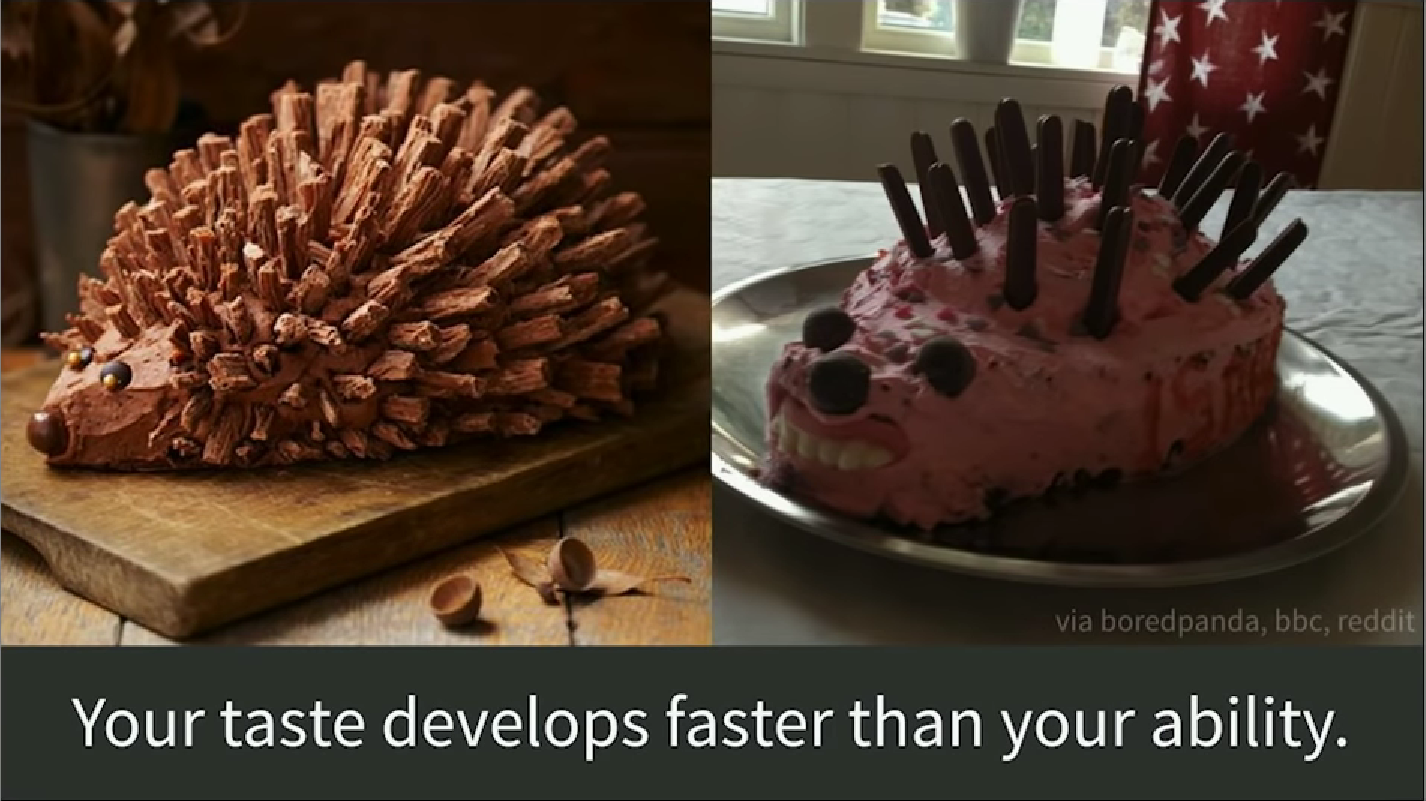
\includegraphics[width=0.95\linewidth]{figures/hedgehog.png}
\end{figure}
Source: \url{https://www.youtube.com/watch?v=7oyiPBjLAWY&t=448s&ab_channel=RConsortium}
\end{frame}

\begin{frame}{What They Forgot (WTF!!!)}
\vspace{-0.75cm}
\begin{itemize}
\itemsep 2ex
\item Always start R with a blank state!
\item Adopt a project-oriented workflow. 
\item Practice safe ``paths". 
\item Work and share examples in a reproducible environment, a so-called \href{https://reprex.tidyverse.org/}{\texttt{reprex}} (see Unit 2). 	
\end{itemize}

\vspace{0.5cm}

The examples are taken from \url{https://rstats.wtf/}. Another course on similar topics (not R-based and slightly more advanced): \url{https://missing.csail.mit.edu/}. 
\end{frame}

\begin{frame}{Always start R with a blank state!}
\vspace{-0.5cm}
\begin{itemize}
\itemsep 3ex
\item By default, when you terminate an R session, the software asks you if you want to save the current workspace. 
\item Similarly, the R startup mechanism\footnote{See also \texttt{?Startup} and \texttt{?quit} for more details.} loads a saved image of the user workspace (i.e. a \texttt{.Rdata} file) if there is one. 
\item Unfortunately, this behaviour might be really dangerous, especially if you don't remember how the saved objects were generated. Citing the Python's style guide PEP20: \textit{Explicit is better than implicit}.  
\end{itemize}
\end{frame}

\begin{frame}{or, as Beyoncé said ...}
\vspace{-0.5cm}
\begin{figure}
\centering

\includegraphics[width=\linewidth]{figures/rihanna.jpg}
\end{figure}
\end{frame}

\begin{frame}{So what can I do?}
\vspace{-0.5cm}
\begin{itemize}
\itemsep 2ex
\item If you run R from the shell, use \texttt{R --no-save --no-restore-data}.
\item In Rstudio, set the following options via Tools -> Global Options.  
\vspace{1.5ex}
\begin{figure}
\centering
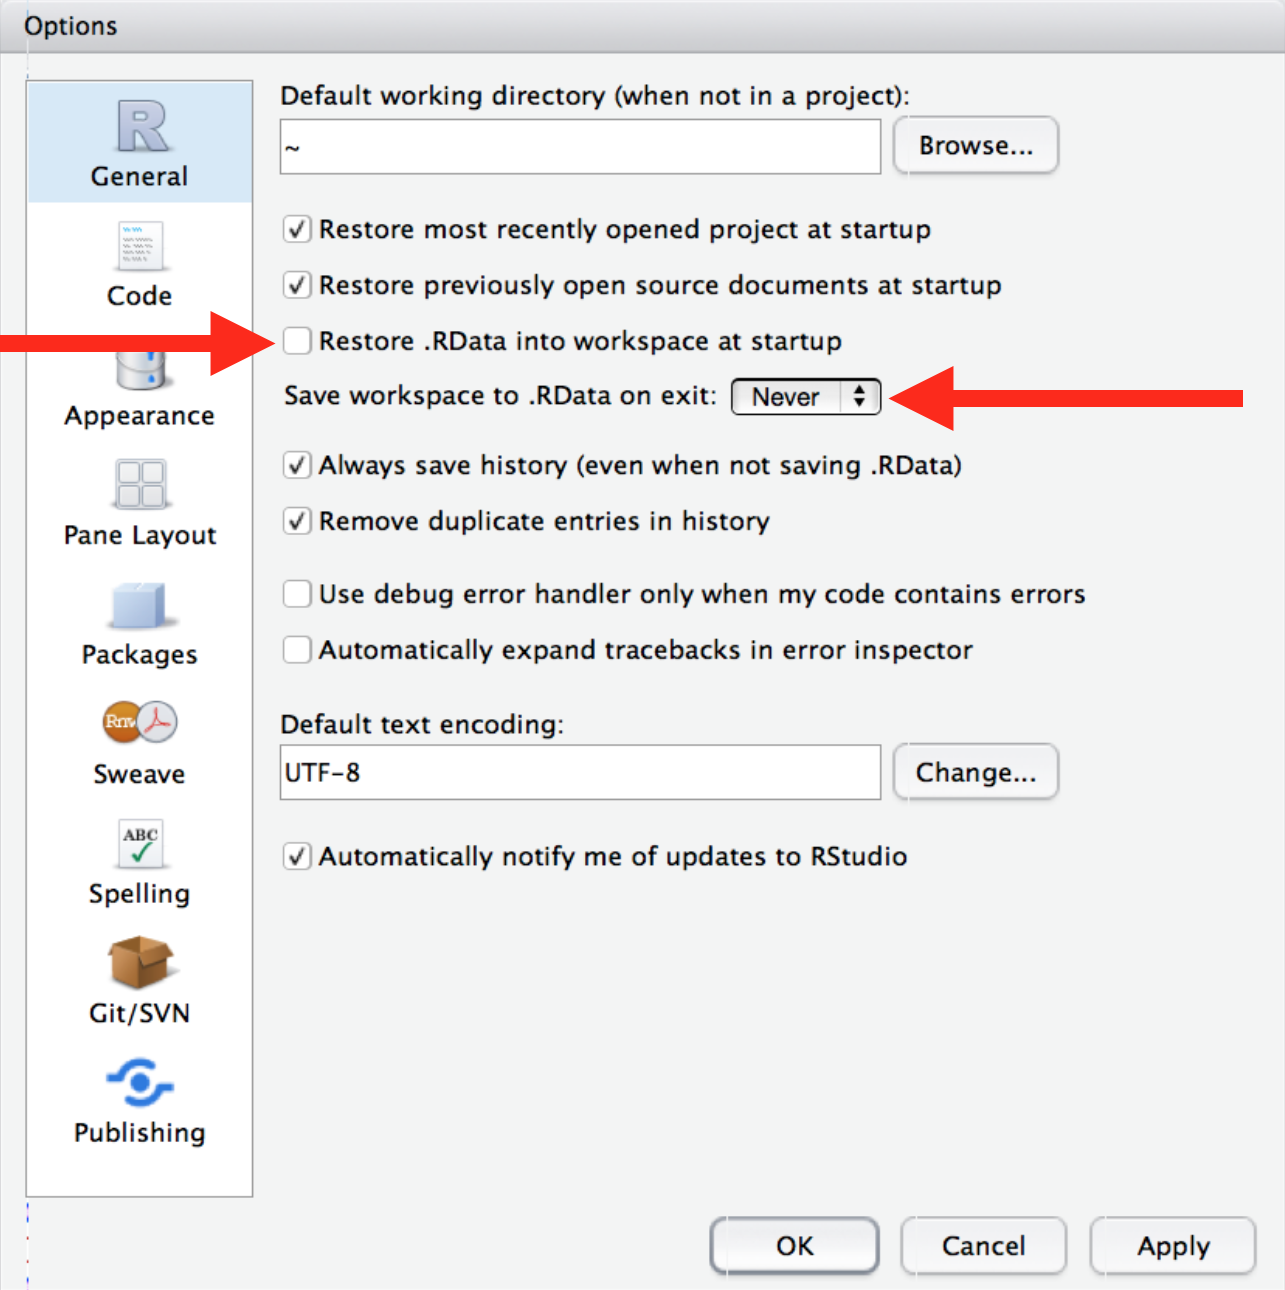
\includegraphics[width=0.9\linewidth, trim=0 13.25cm 0 0, clip]{figures/rstudio-workspace.png}
\end{figure}
\end{itemize}
\end{frame}

\begin{frame}{Adopt a project-oriented workflow}
\vspace{-0.5cm}
\begin{itemize}
\itemsep 2ex
\item There are many R scripts that begin with the following lines: 
\begin{itemize}
\item \texttt{rm(list = ls())} \texttt{\# "clean" the environment}
\item \texttt{setwd("path/that/I/only/have")} \texttt{\# adjust the wd}
\end{itemize}
\item What is the problem with the previous code chunks? 
\begin{itemize}
\item \texttt{rm(list = ls())} is not enough to properly clean your R session. Let's see an example! 
\item The previous \texttt{setwd(...)} command is (almost surely) going to fail for everyone who is not the original user \emoji{sad-but-relieved-face}
\end{itemize} 
\vspace{0.5ex}
\end{itemize}
{\Huge$\Longrightarrow$} Organise your analyses as independent (Rstudio) projects, each belonging to a separate folder. Let's try! 
\end{frame}

\begin{frame}{Adopt a project-oriented workflow}
\begin{figure}
\centering
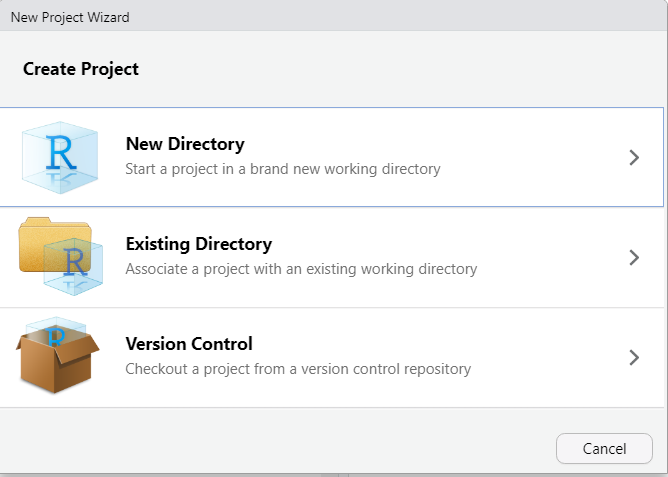
\includegraphics[width=0.9\linewidth]{figures/rstudio-proj.png}
\end{figure}
\end{frame}

\begin{frame}{Practice safe ``paths"}
\vspace{-0.5cm}
\begin{itemize}
\itemsep 3ex
\item Why do we usually run \texttt{setwd(...)}? Because we want to specify the "relative" path of a file according to a directory. 
\item Unfortunately, \texttt{setwd(...)} may raise several portability issues as seen before. 
\item The \href{https://here.r-lib.org/}{\texttt{here}} \emoji{package} provides a convenient way to perform the same operation without manual interventions and the aforementioned drawbacks $\Longrightarrow$ Practice safe ``paths""! 
\item Let's see an example and more details!
\end{itemize}
\end{frame}

\begin{frame}
\vspace{2cm}
\begin{center}
\Huge
\textbf{The tidyverse!}
\end{center}
\vspace{1.5cm}
\epigraph{The tidyverse is a set of packages that work in harmony because they share common data representations and API design.}{\url{https://tidyverse.tidyverse.org/}}
\end{frame}

\begin{frame}{EDA with the Tidyverse}
\vspace{-0.5cm}
We are going to briefly showcase the tidyverse toolkit using a series of relational dataset obtained from \href{https://www.data.gov.uk/dataset/cb7ae6f0-4be6-4935-9277-47e5ce24a11f/road-safety-data}{here}.
\begin{figure}
\centering
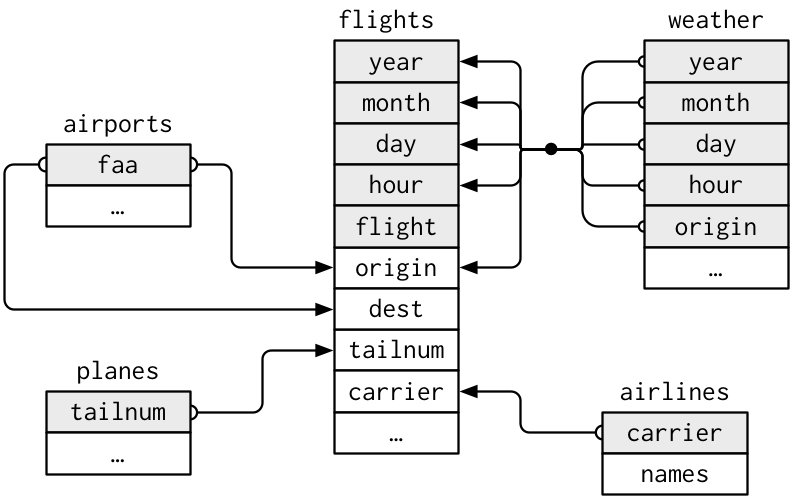
\includegraphics[width=0.8\linewidth]{figures/relational-nycflights.png}
\end{figure}
{\small Source: \url{https://r4ds.had.co.nz/relational-data.html}.}
\end{frame}

\begin{frame}
\vspace{2cm}
\begin{center}
\Huge
\textbf{Enough theory, let's start coding \emoji{partying-face}}
\end{center}
\end{frame}
\end{document}